%Aysha's sections + Darius's application subsection
\section{Introduction}

%aysha to do
%change figures to pdfs. same size font and same font.

\subsection{Classical Hall Effect}
The classical Hall effect is a consequence of charged carriers moving in a magnetic field. The setup involves, a magnetic field $\vec{B}$ in the z-direction, charged carriers restricted in the (x,y)-plane, and a constant current $I$ flowing in the x-direction, illustrated in Fig. \ref{classical-hall-effect}. The motion of the charged carriers induces a voltage $V_H$ in the y-direction, named the Hall voltage after Edwin Hall who discovered the effect in 1879 \cite{tong_notes}.

\begin{figure}[h!]
    \centering
    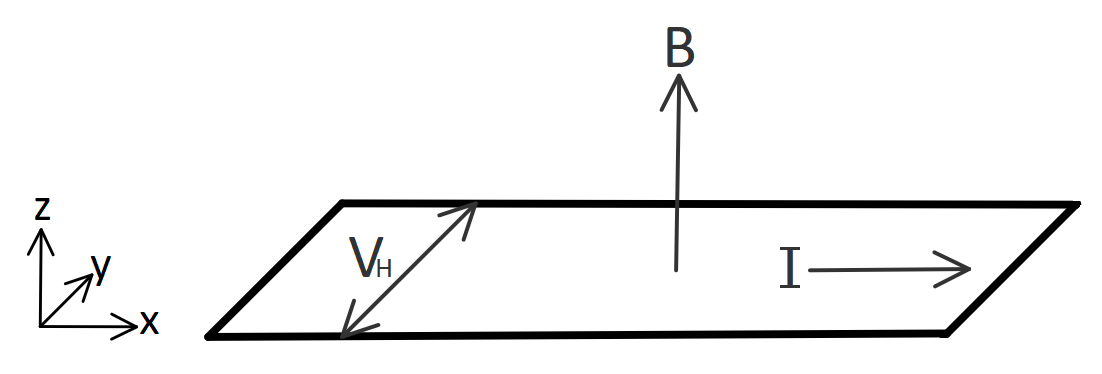
\includegraphics[width=7cm]{figures/hall effect set up.png}
    \caption{Hall effect set up.} 
    \label{classical-hall-effect}
\end{figure}

The Drude model predicts an equation of motion for a particle of mass $m$ and charge $-e$ in a magnetic field $\vec{B} = B\uvec{z}$ with velocity $\vec{v} = \dot{x}\uvec{x} + \dot{y}\uvec{y}$,
\begin{equation}
    m \frac{d\vec{v}}{dt} = -e(\vec{E} + \vec{v} \times \vec{B}) - \frac{m\vec{v}}{\tau}
\end{equation}
where the electric field produced by the current $\vec{E} = E\uvec{x}$ and the last term is the linear friction term, with $\tau$ being  the scattering time. 

The current density $\vec{J}$,
\begin{equation}
    \vec{J} = \sigma \vec{E}
\end{equation}
This is known as Ohms law, where $\sigma$ is the conductivity matrix.

\begin{equation}
    \sigma = 
    \begin{pmatrix}
    \sigma_{xx} & \sigma_{xy}  \\
    -\sigma_{xy} & \sigma_{xx} 
    \end{pmatrix}
\end{equation}

The resistivity is defined as the inverse of the conductivity,
\begin{equation}
    \rho = \sigma^{-1} =
    \begin{pmatrix}
    \rho_{xx} & \rho_{xy}  \\
    -\rho_{xy} & \rho_{xx} 
    \end{pmatrix}
\end{equation}

The model makes the experimental predictions that the longitudinal resistivity $\rho_{xx}$ and the Hall resistivity $\rho_{xy}$ should be 
\begin{equation}
    \rho_{xx} = \frac{m}{n e^{2} \tau} \mbox{ and } \rho_{xy} = \frac{B}{ne}
\end{equation}
where $n$ is the electron density. These relations are shown in Fig. \ref{classical-resistivities}.

\begin{figure}[h!]
    \centering
    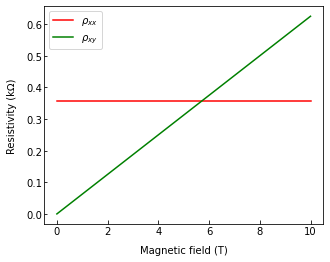
\includegraphics[width=7cm]{figures/classical hall effect rhovsB 2.png}
    \caption{The classical hall effect expectation with $n= 10^{17} m^{-3}$ and $\tau = 10^{-12} s$.}
    \label{classical-resistivities}
\end{figure}

\subsection{Quantum Hall Effect}
The classical theory no longer becomes a reliable theory to use once we enter the quantum regime, i.e at low temperatures and high magnetic fields. The Quantum Hall effect was first discovered experimentally. 

\begin{figure}[h!]
    \centering
    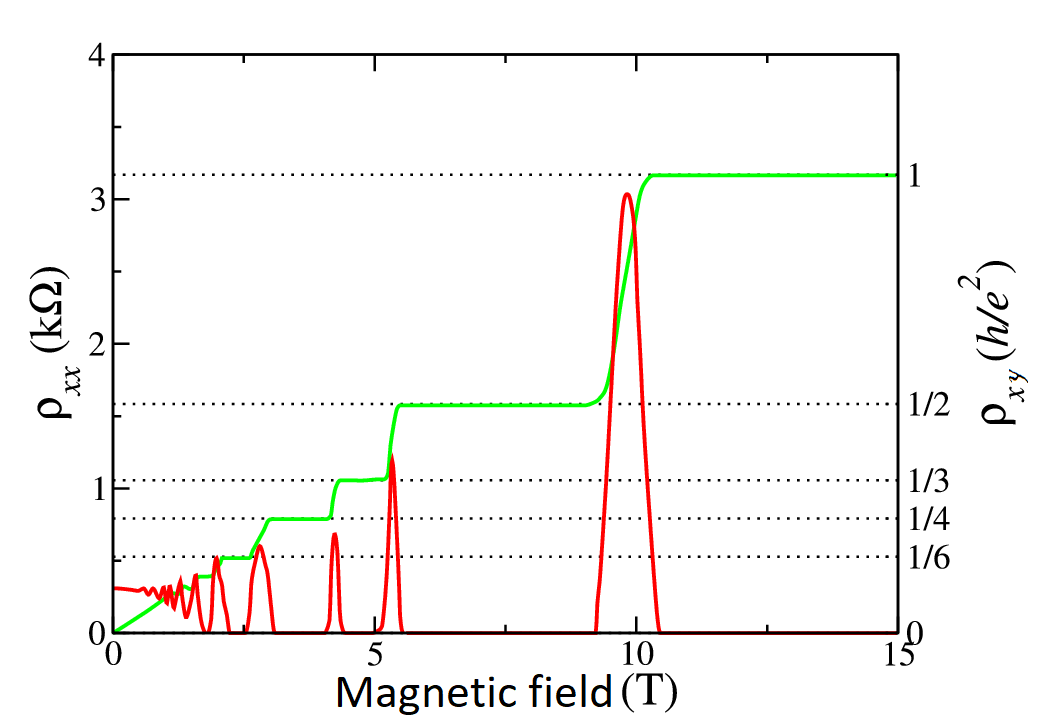
\includegraphics[width=7cm]{figures/quantum hall effect rhovsB.png} 
    \caption{The quantum Hall effect expectation. Figure taken from \cite{qhe-plot}}
    \label{quantum-hall-res}
\end{figure}

Klaus von Klitzing performed the first experiments to observe the quantum regime of the Hall effect in 1980 \cite{klitz_method}. In Fig \ref{quantum-hall-res} the Hall resistivity and longitudinal resistivity exhibit behaviour not expected or explained by the classical Hall effect. The Hall resistivity lies on a plateau for a range of magnetic fields, before jumping to the next plateau. For each plateau, the resistivity is quantized and takes the form
\begin{equation}
    \rho_{xy}= \frac{2 \pi \hbar}{e^2} \frac{1}{\nu} \ \ \nu  \in \mathbb{Z}
\end{equation}

The integer $\nu$ is measured to remarkable accuracy, which means it can be used to measure the ratio of fundamental constants $\frac{2 \pi \hbar}{e^2}$ \cite{qhe-res}.

The central plateaux occur when the magnetic field is,
\begin{equation}
    B = \frac{2 \pi \hbar n}{\nu e} = \frac{n}{\nu} \phi_{0},
\end{equation}
where $\phi_{0}= 2 \pi \hbar / e$ is the flux quantum. The values of the magnetic field are the values such that the first $\nu  \in  \mathbb{Z}$ Landau levels are filled.

These plateaux originate from disorder within the experiment. The more disorder, the more prominent the plateaux are. 


\subsection{Motivation and Applications}

The discovery of QHE revolutionized solid-state physics. Where classical Hall resistivity is a linear function of the magnetic field, Quantum Hall resistivity reveals quantized plateaus that are a function of magnetic field. This quantization is independent of microscopic details of the system as such, the QHE has found uses in metrology and calibration \cite{Metrology}. The Plateaus can be used as a calibration for resistance as they exist as one over integer multiples of $\frac{2 \pi \hbar}{e^2}$ accurate to around 8 in $10^{11}$ \cite{doi:10.1063/1.2776371}. This defines the Von Klitzing constant $R_k$ which takes the value of $25,812.80745\Omega$. From 1991 until
when SI units were redefined in 2018, This was how the Ohm was defined. Equipment was calibrated such that when measuring quantum hall resistivities, the plateaus would exist at one over integer multiples of $R_k$. 

The QHE, as will be seen, is liked to topology and topological invariants \cite{tong_notes}. These are intrinsic properties of a system that cannot be changed under continuous transformations in the parameters of the system. QHE was the first observed manifestation of topological invariants influencing the measurable properties of a system and led to whole new research into topological phase transitions \cite{RevModPhys.82.3045}. One example of this is the topological insulator which is a material that acts as an insulator but has metallic chiral edge states \cite{Moore2010}. Chiral edge states meaning that all electrons traveling in one direction along the materials edge have a particular spin (spin up) and those traveling in the opposite direction have opposite spin (spin down) with the directions reversed on the opposite edge as in fig.\ref{top_insulator} While the QHE appears as a result of an external magnetic field, Topological insulators are a result of spin-orbit coupling within the material so in essence, it is the internal magnetic field of the materials. 

\begin{figure}[h!]
    \centering
    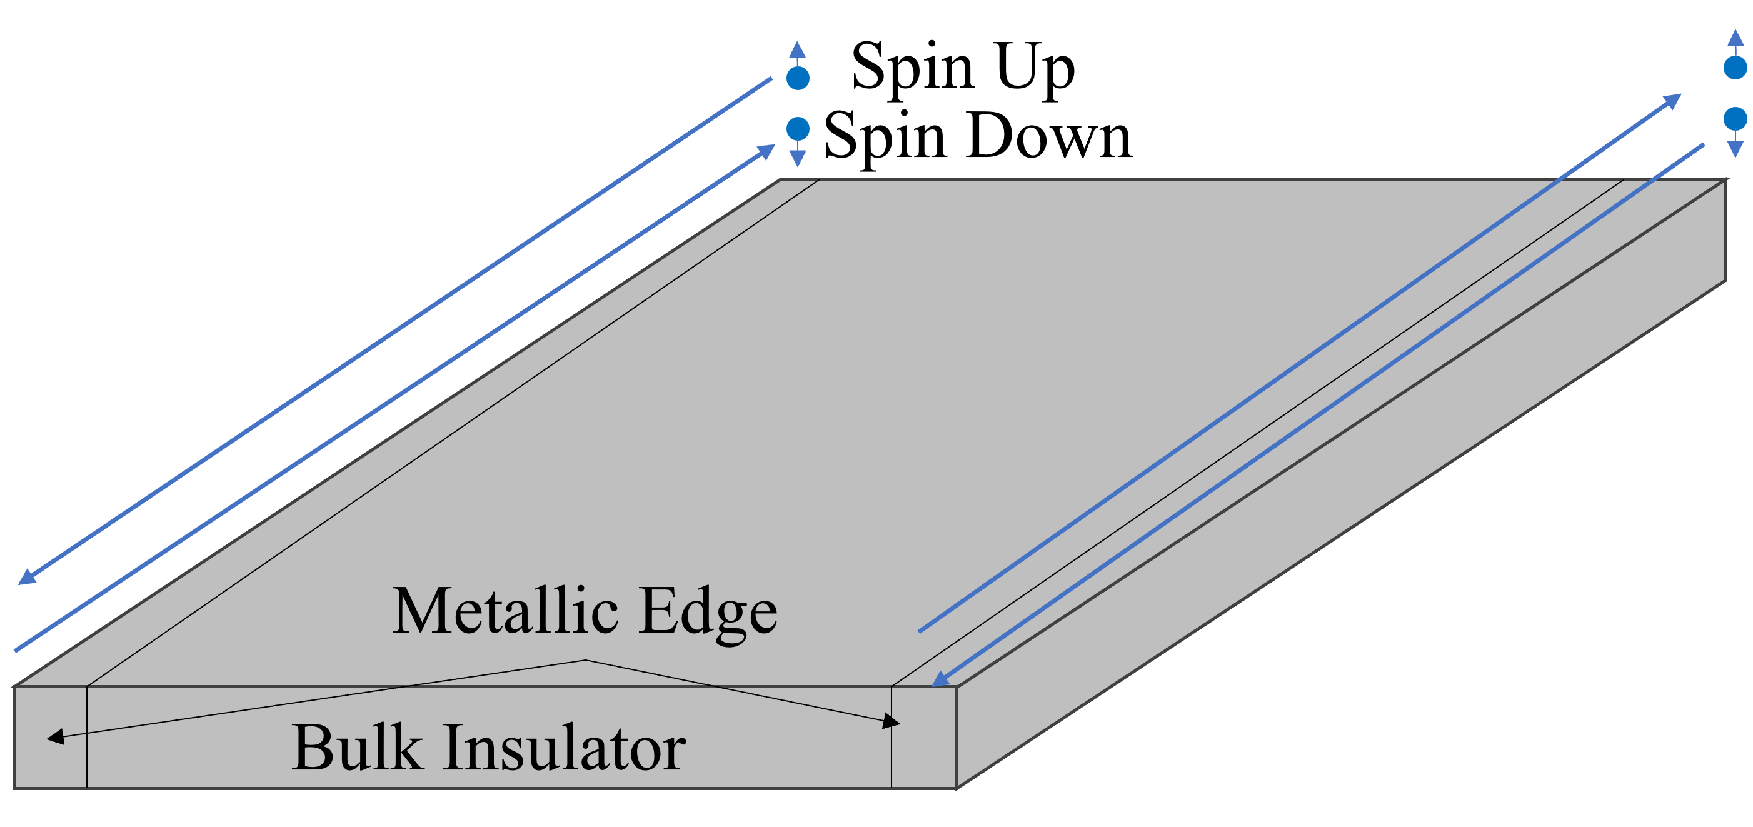
\includegraphics[width=8cm]{figures/top_insulator.pdf}
    \caption{Illustration of the chiral nature of the edge states of a 2D topological insulator. }
    \label{top_insulator}
\end{figure}
